\documentclass[oneside,10pt]{book}

\usepackage{cdtBook}
\usepackage{usecases}
\usepackage{gensymb}

\title{ProjectADOO}
\subtitle{E-IMSS}
\author{Black::Sheep()}


%%%%%%%%%%%%%%%%%%%%%%%%%%%%%%%%%%%%%%%%%%%%%%%%%%%%%%%%%%%%%%%%
\begin{document}

\maketitle
\thispagestyle{empty}


\tableofcontents



%=========================================================
\chapter{Introducción}

\cfinput{Introduccion/Introduccion}

%=========================================================
\chapter{Análisis del problema}

\cfinput{Analisis/Problematica}

%=========================================================
\chapter{Propuesta de solución}

\cfinput{Propuesta/Propuesta}



%=========================================================
\chapter{Modelo de Negocios}

\cfinput{ModeloNegocios/brGlosario}
\cfinput{ModeloNegocios/brProceso}
\cfinput{ModeloNegocios/brModelo}
\cfinput{ModeloNegocios/brReglas}

%=========================================================
\chapter{Modelo del despliegue del sistema}
\cfinput{ModeloDespliegue/ModeloDespliegue}

%=========================================================
\chapter{Modelo de comportamiento}
	
	\begin{figure}[htbp!]
		\centering
			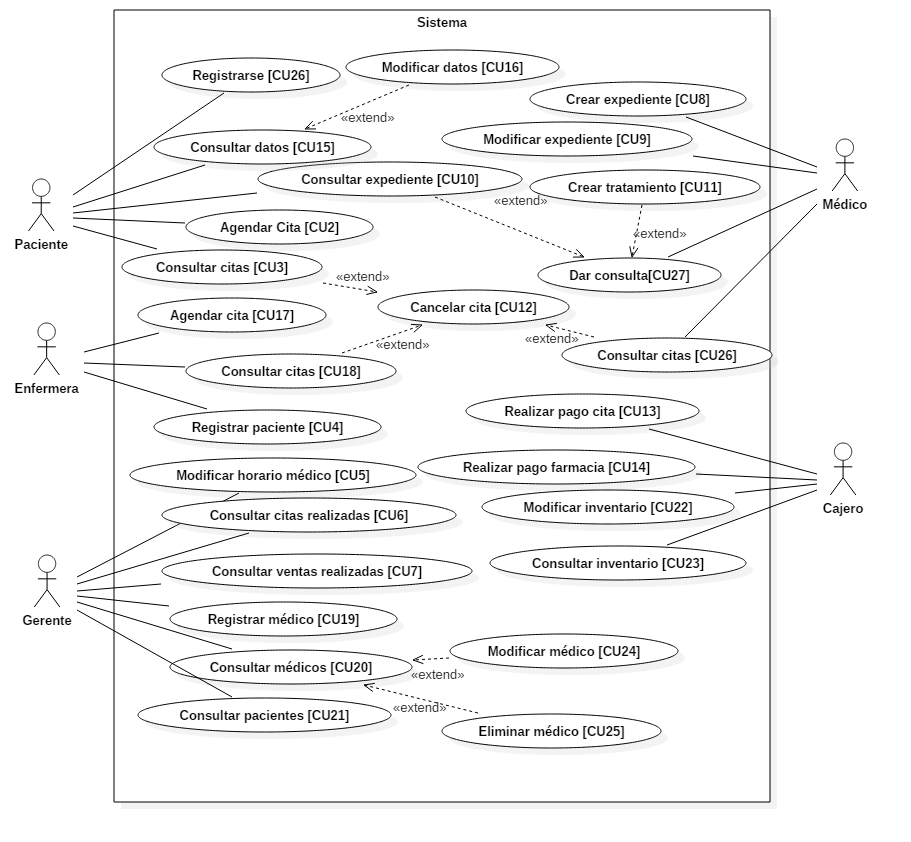
\includegraphics[width=1.1\textwidth]{images/Diagrama_CU_general}
		\caption{Diagrama de casos de uso del sistema.}
	\end{figure}
	
%\cfinput{ModeloComportamiento/cu}
\cfinput{ModeloComportamiento/AgendarCita/AgendarCita}
\cfinput{ModeloComportamiento/ConsultarCitas/ConsultarCitas}
\cfinput{ModeloComportamiento/ConsultarPacientes/ConsultarPacientes}
\cfinput{ModeloComportamiento/CrearExpediente/CrearExpediente}
\cfinput{ModeloComportamiento/ConsultarExpediente/ConsultarExpediente}
\cfinput{ModeloComportamiento/CrearTratamiento/CrearTratamiento}
\cfinput{ModeloComportamiento/ModificarHorarioMedico/ModificarHorarioMedico}
\cfinput{ModeloComportamiento/RealizarPagoCita/RealizarPagoCita}
\cfinput{ModeloComportamiento/RealizarPagoFarmacia/RealizarPagoFarmacia}
\cfinput{ModeloComportamiento/RegistrarPaciente/RegistrarPaciente}
\cfinput{ModeloComportamiento/ModificarInventario/ModificarInventario}
\cfinput{ModeloComportamiento/ConsultarInventario/ConsultarInventario}


%%=========================================================
\chapter{Modelo de la Interacción}

%\cfinput{ModeloInteraccion/navegacion}
\cfinput{ModeloInteraccion/Adrian/IU}
\cfinput{ModeloInteraccion/Demis/IU}
\cfinput{ModeloInteraccion/Murga/IU}
\cfinput{ModeloInteraccion/Pacheco/IU}
\cfinput{ModeloInteraccion/Trujillo/IU}
%\cfinput{ModeloInteraccion/IU23}
%\cfinput{Pantallas/IU1}
%\cfinput{Pantallas/IU2}
%\cfinput{Pantallas/IU3}
%\cfinput{Pantallas/IU4}
%\cfinput{Pantallas/IU5}
%\cfinput{Pantallas/IU6}
%\cfinput{Pantallas/IU7}

	
\end{document}
